\subsection{Evaluating Performance Comparison Results}
\label{subsec:evaluating_PerfomanceComparison}

%\textbf{COHEN: How did the program performance compare to its selected standard?} 
%\textbf{Did the program demonstrate good performance?}
%\textbf{Is the programs performance different from predictions?} 
%\textbf{Did you learn what you wanted from the experiments?}

The best route set, having four routes, constructed by the proposed method (SSO), is presented in Table \vref{table:performanceComparison_bestRouteSet4} and illustrated in Fig. \vref{fig:bestRouteSet4}. The best route set, having four routes, constructed by a plain ACO implementation is found in Table \vref{table:performanceComparison_bestRouteSet4_ACO}. The best, worst, average, median produced results with the standard deviation can be found in Appendix \ref{appendixC}, Table \vref{table:performanceComparison_ACOFull}. 

The SSO is as mentioned in Section \vref{subsec:performanceComparison_setup}, identical to the plain ACO implementation, but with the additional attributes inspired by PSO and BCO, in addition to the memory attribute. By using an otherwise identical algorithm enables directly comparing the performance of the two algorithms. As one can see in Table \vref{table:performanceComparison_ACOSSOBEST}, SSO performs better than ACO concerning the performance criteria. 

Observing Figure \ref{fig:acovssso}, the ACO performs worse than SSO already in the first iteration. A reason for this is that the ants in ACO does not possess the memory attribute. This feature enables ants to ``remember'' which nodes it has visited within the same route set. Adding this attribute makes the ants favor nodes not visited over nodes already visited, to make sure all nodes are visited within the same route set. Constraint \vref{itm:criteriaConnectedGraph} specifies that the route network must be connected, and without the memory function, ACO will produce more route networks not satisfying the constraint. This again makes ACO produce route sets that will be discarded, and not evaluated. %The lack of this attribute will thus prevent more (possible better) route sets being explored.  

 \begin{figure}[H]
    \begin{center}
    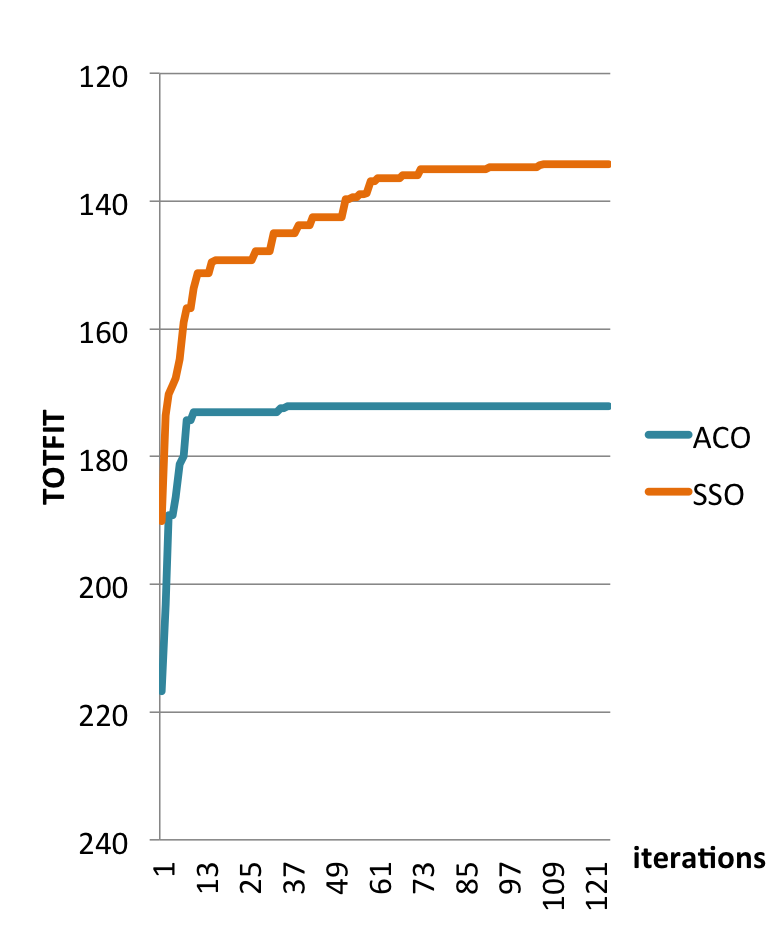
\includegraphics[width=2.5in]{assets/acovsssoNEW.png}
    \end{center}
    \caption{Evolution of TOTFIT for ACO and SSO }
    \label{fig:acovssso} 
\end{figure}

Another reason for the performance difference is that ACO also has, as mentioned, a known limitation of getting stuck at a local optima. This disadvantage is demonstrated in Figure \ref{fig:acovssso}, which shows the average growth in the $TOTFIT$ value for each iteration. Both algorithms are run 10 times, and for each iteration the average $TOTFIT$ value for each run is recorded. As one can observe, the ACO implementation manage to find good solutions fast, by following pheromone trails laid by previous ants. However, after approximately 35 iterations, the algorithm does not discover better solutions. The amount of pheromone on the initial first best routes continue to increase, and with this, unable the next ants to explore possible better routes. 

As one can see, the proposed SSO algorithm manage to get out of this inconvenience. As observed in the parameter settings experiment, summed in Table \vref{table:pm2_inEvaluation}, the additional $CA$ and $AF$ parameters both improve the $TOTFIT$ value. The experiments were conducted to find the optimal value for these parameters. %It is worth mentioning, the experiments performed in this table was done in order to find the best parameter value for the algorithm performance, and the default value while testing for both parameters was 10\%.
The amount of $CA$ enables the algorithm to explore new (possible better) routes, regardless of the pheromone value laid on the edges. This parameter can therefore enable the algorithm to get out of a local optima. The reader recalls that the $AF$ parameter selects and amount of the best produced route sets of an iteration, and the following ants will basically reward these edges with more pheromone. Giving these edges additional pheromone by the $p_b$ parameter improved the algorithms performance further. Rewarding edges in a large amount best route sets will result in over appreciating too many edges, which again will unable to distinct edges in good route sets from edges in the best route sets.

\begin{table}
    \centering
    %\hspace*{-0.5cm}
    \begin{tabular}{|l|l|l|l||c|}
    \hline
    Parameter & $CA$ & $AF$ & $p_b$ & $AVG(TOTFIT)$ \\
    \hline
    $CA$ & \textbf{0\%} & 10\% & 0.0 & 105.66\\
    ~ & \textbf{25\%} & 10\% & 0.0 & \textbf{103.597}\\
    \hline
    $AF$ & 10\% & \textbf{0\%} & 0.0 & 105.747 \\
    ~ & 10\% & \textbf{5\%} & 0.0 & \textbf{104.389}\\
    \hline
    $p_b$ & 10\% & 5\% & \textbf{0.0} & 104.882\\
    ~ & 10\% & 5\% & \textbf{0.9} & \textbf{102.579}\\
    \hline
    \end{tabular}
    \caption {Caption}
    \tiny
    \begin{itemize}[noitemsep]
    \item[ ] $AVG(TOTFIT)$ : Average produced Total Fitness function
    %\item[$^1$:] On average \% of the iterations of each run did not create any ants that satisfied the initial Constraint \ref{itm:criteriaConnectedGraph} described in Section \vref{sec:algoConstraints}.
    \end{itemize}
    \label{table:pm2_inEvaluation}
\end{table}

%TODO:
%The ants in SSO also possess the knowledge of the global best known solution. This feature will increase the probability of the next ants selecting the edges walked by the best ant so far. Further, if a better global best known solution is found, new edges will have increased probability of being selected, and the next ants will walk towards a better global solution. As one can see in \vref{table:performanceComparison_ACOSSOGlobal_sol}, this did not improve the SSO algorithm further. 

In Table \vref{table:performanceComparison_4}, the results of the SSO, having four routes, are compared with route sets published in the literature. As one can observe in Table \vref{table:performanceComparison_4}, all approaches compared to, except \citep{mandl79, kidwai98, chakroborty02}, produce better route sets concerning the $d_0$ criteria. However, the route set constructed by SSO has a lower $ATT$ compared to all route sets constructed by the other approaches. 

The calculation of $TOTFIT$ is, as mentioned, the sum of $F1$, $F2$ and $F3$. As described in \vref{sec:f1}, a weight parameter, $\sigma$, is used to control the importance of $F1$, $F2$, and $F3$. In the proposed algorithm, $\sigma$ is sat to favor $F1$, which is directly linked to a low $ATT$. Demonstrated in Fig. \vref{fig:mandlWithTT}, when traveling from node 7 to node 14 the algorithm will choose to transfer from route 4 to route 3, and the total travel time will be 20 minutes including a transfer penalty of 5 minutes. The $F2$ parameter is concerned whether the algorithm has a high $d_0$, denoting a minimum number of transfers. If $F2$ is favored over $F1$, route 1, which have a direct route from node 7 to node 14, would be selected. The travel time for this route is 27 minutes, increasing the $ATT$. It is worth mentioning that the algorithm does not select $F1$ unconditionally, a high amount of $d_0$ is still important, but the algorithm select the best route set concerning the ratio between the two. The theoretical best value of $F3$ is 0, which reflects no passenger have to transfer more than 2 times. \emph{\color{blue} TODO: evaluate}

\begin{figure}[H]
    \begin{center}
    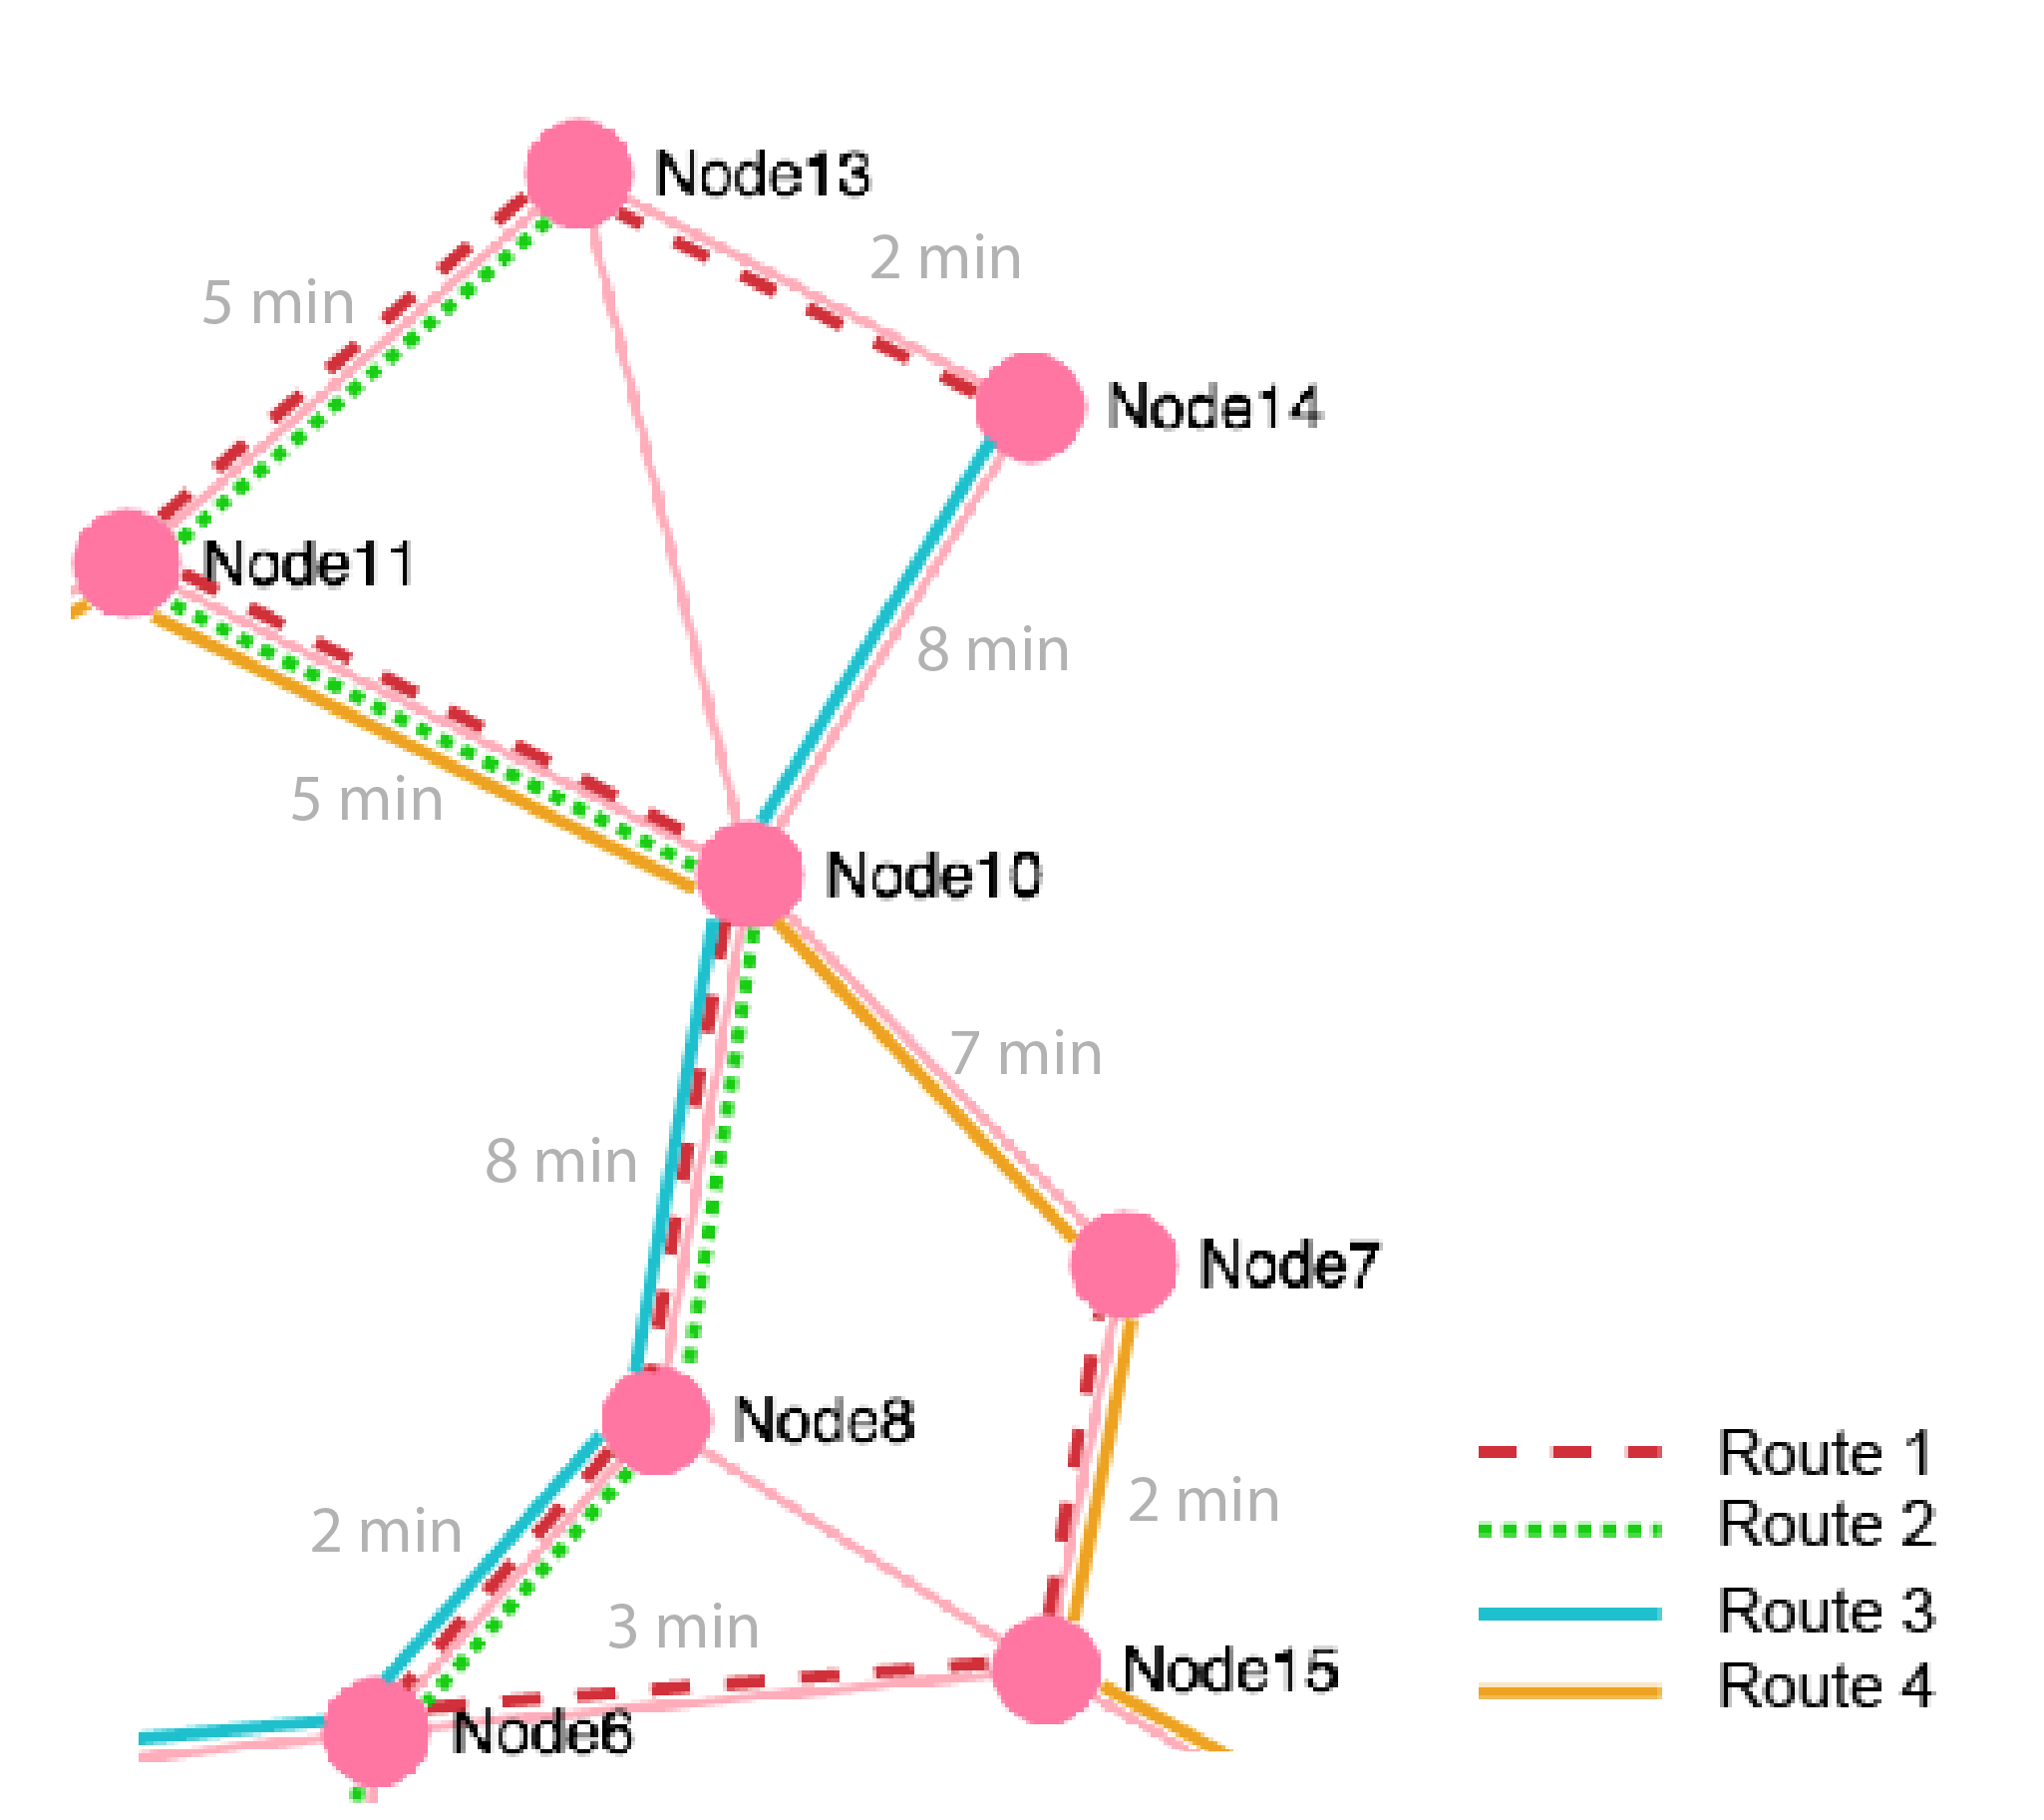
\includegraphics[width=3.5in]{assets/mandl_withTT_utsnitt.png}
    \end{center}
    \caption{A fragment of the best route set, having four route sets, constructed by the proposed algorithm including transfer times in minutes between each node.}
    \label{fig:mandlWithTT} 
\end{figure}

The best route set, having six routes, constructed by the proposed algorithm is presented in Table \vref{table:performanceComparison_bestRouteSet6} and Fig. \vref{fig:bestRouteSet6}.  The best route set, having seven routes, constructed by the proposed algorithm is presented in Table \vref{table:performanceComparison_bestRouteSet7} and Fig. \vref{fig:bestRouteSet7}. The best route set, having eight routes, constructed by the proposed algorithm is presented in Table \vref{table:performanceComparison_bestRouteSet8} and Fig. \vref{fig:bestRouteSet8}. As one can observe from these tables, the proposed algorithm still has a higher $ATT$ than all other approaches. The performance criteria, $d_0, d_1, and d_{2}$ are all still below average, and $d_{unsat}$ are the same. \emph{\color{blue} TODO: evaluate}

As one can observe in \vref{table:performanceComparison_routesets}, the amount of direct travelers increase in line with the number of route sets. This makes sense because thus more route sets the passengers can choose from, thus bigger probability for the passenger finding a convenient route. \emph{\color{blue} TODO: evaluate} 

 \begin{table}[H]
    \centering
    \begin{tabular}{|l||l|l|l|l|l|}
    \hline
    Route Set & $d_0(\%)$ & $d_1(\%)$ & $d_2(\%)$ & $d_{unsat}(\%)$ & $ATT$ \\
    \hline
    4 & 85.21 & 13.49 & 1.30 & 0.00 & 10.27\\
    6 & 87.17 & 12.0 & 0.82 & 0.01 & 10.11\\
    7 & 88.49 & 10.72 & 0.79 & 0.0 & 10.08\\
    8 & 89.16 & 10.05 & 0.80 & 0.0 & 10.06\\\\
    \hline
    \end{tabular}
    \caption {Evaluating increase of Route Sets}
    % 50 runs
    \label{table:performanceComparison_routesets}
\end{table}

